% Created 2023-11-11 Sat 22:57
% Intended LaTeX compiler: xelatex
\documentclass[11pt]{article}
\usepackage{ctex}
\usepackage{graphicx}
\usepackage{grffile}
\usepackage{longtable}
\usepackage{wrapfig}
\usepackage{rotating}
\usepackage[normalem]{ulem}
\usepackage{amsmath}
\usepackage{textcomp}
\usepackage{amssymb}
\usepackage{capt-of}
\usepackage{hyperref}
\author{Kintrol}
\date{\textit{<2023-11-11 Sat>}}
\title{landau}
\hypersetup{
 pdfauthor={Kintrol},
 pdftitle={landau},
 pdfkeywords={},
 pdfsubject={},
 pdfcreator={Emacs 29.1 (Org mode 9.6.6)}, 
 pdflang={English}}
\begin{document}

\maketitle
\begin{figure}[htbp]
\centering
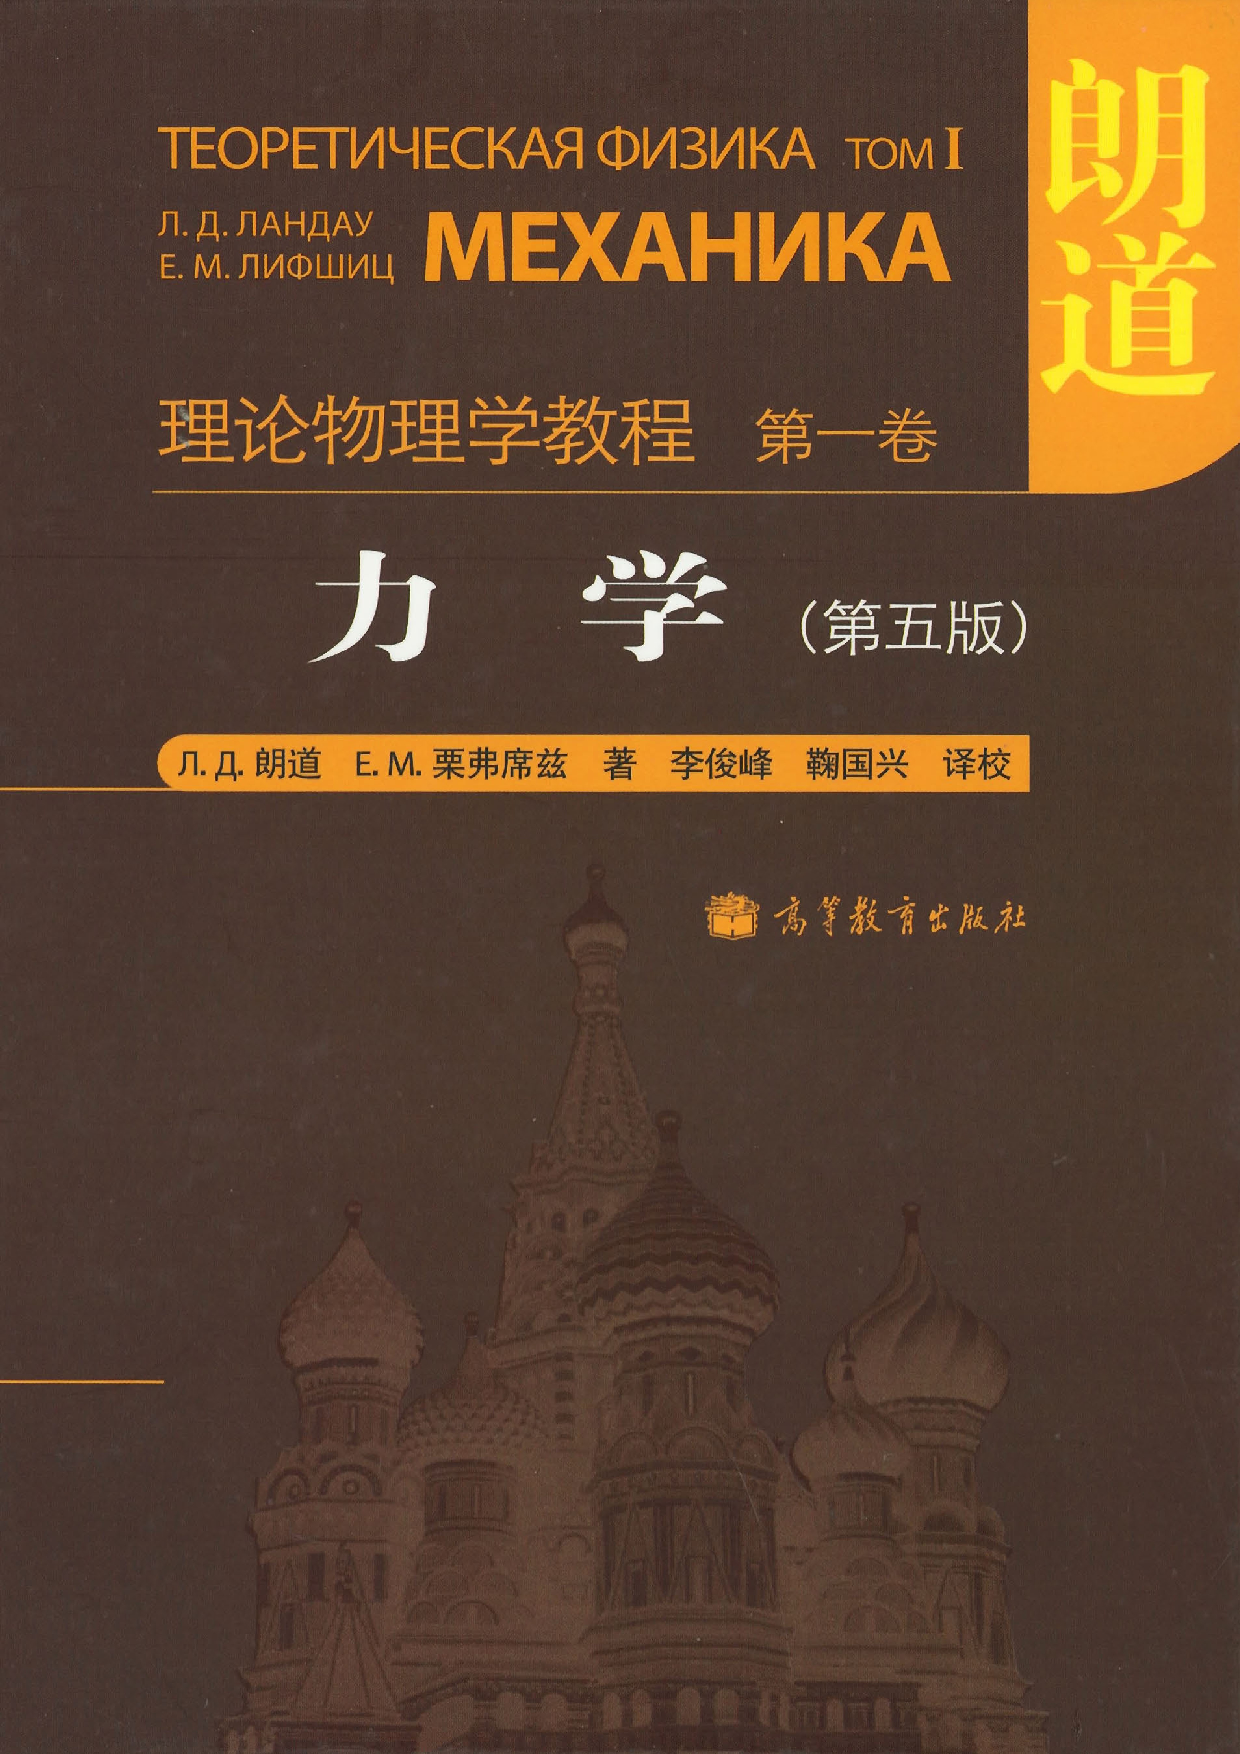
\includegraphics[width=.9\linewidth]{./img/front.pdf}
\caption{Here I come}
\end{figure}

自我学习笔记
\section{运动方程}
\label{sec:org492993d}
\subsection{+ 重点:}
\label{sec:orgbb272b9}
\begin{itemize}
\item 如何得出 Lagrange 函数
\item 自由质点和其他系统有什么区别
\end{itemize}
\subsection{广义坐标}
\label{sec:org20ffa7e}
\begin{itemize}
\item 概念
\end{itemize}

广义坐标 \(q(t)\) \(\rightarrow\) 广义速度 \(\dot{q}(t)\)


\begin{verse}
符号上加点对时间求导/空间?\\[0pt]
\end{verse}

自由度:决定坐标需要的独立变量数目
取自由度个数的(独立)广义坐标描述运动
只需要坐标和速度就可以确定物体运动情况 = 数学可解方程
\begin{verbatim}
这一点是因为牛顿的力学方程吗?因为 $F=ma=m\ddot{x}$ 它会构成二阶方程,因此初值条件是两个(零阶和一阶)
\end{verbatim}

\begin{itemize}
\item 补充:
\item 坐标变换
不变的物理规律
\item 约束【有约束采油所谓自由】
\end{itemize}
即方程。
\begin{enumerate}
\item (非)定常:方程是否显含时间
\item (非)理想:虚功和为0 \(\sum F\cdot\delta r =0\),举例:光滑接触不可伸长、铰链、刚性杆
\begin{verbatim}
不懂?
\end{verbatim}
\item (不)完整:完整只限制位置,非限制速度
\item (单)双侧:方程是(不等式)等式
\end{enumerate}
\subsection{最小作用量}
\label{sec:org16815e7}
力学函数/Lagrande 函数: 直接假想定义有一个普遍的力学函数,由最小作用量原理我们认定每个力学系统可以用一个确定的函数描述。性质特殊
\begin{equation}
\label{eq:defL}
L(q_i,\dot{q}_i,t)
\end{equation}
作用量: \(L\) 对时间积分
\begin{equation}
\label{eq:defS}
S := \int\limits_{t_2}^{t_1}L(q,\dot{q},t)\mathrm{d}t
\end{equation}
最小作用量原理/Hamilton 原理:
\(S\) 取最小

变分法

\begin{verbatim}
Landau 这里根本没提变分,只是说取一个很小量,使得过程很自然(可能对不料这后面显得优点难懂)
\end{verbatim}

\sout{考虑微小变化}
如果取价值那么使用任何的 \(q(t)+\delta q(t)\) 都会使得 \(S\) 增大,
我们认为 \(\delta q(t)\) 是小量,于是
\begin{equation}
\label{eq:3}
\delta q(t_1)=\delta q(t_2)
\end{equation}
?研究这个增量带来的变化
\begin{equation}
\label{eq:1}
S'- S = \int\limits_{t_2}^{t_1}L(q+\delta q,\dot{q}+\delta \dot{q},t)\mathrm{d}t - \int\limits_{t_2}^{t_1}L(q,\dot{q},t)\mathrm{d}t
\end{equation}  
极值点要求 \(\delta S=0\)
于是
\begin{equation}
\label{eq:2}
\int\limits_{t_2}^{t_1}(\frac{\partial L}{\partial q}\delta q+\frac{\partial L}{\partial \dot{q}})\mathrm{d}t=0
\end{equation}

\begin{verbatim}
?为什么不对时间求
因为上面
\end{verbatim}

对第一项作分步积分
\begin{equation}
\label{eq:7}
\delta L=\frac{\partial L}{\partial q}\delta q+\frac{\partial L}{\partial \dot{q}}\delta \dot{q}
\end{equation}
有
\begin{equation}
\label{eq:8}
\delta \dot{q}=\frac{\mathrm{d}}{\mathrm{d}t}\delta q
\end{equation}

于是
\begin{equation}
\label{eq:9}
\delta L =\frac{\partial L}{\partial q}+\frac{\mathrm{d}}{\mathrm{d}t}\frac{\partial L}{\partial \dot{q}}\delta q
\end{equation}


\begin{equation}
\label{eq:4}
\delta S=\frac{\partial L}{\partial \dot{q}}\big|^{t_2}_{t_1}+\int\limits_{t_2}^{t_1}(\frac{\partial L}{\partial q}-\frac{\mathrm{d}}{\mathrm{d}t}\frac{\partial L}{\partial \dot{q}})\delta q\mathrm{d}t=0
\end{equation}
\begin{verbatim}
认为 $\frac{\partial L}{\partial q}$ 是常量
\end{verbatim}

第一项由
(\ref{eq:3})
得到为0

考虑到对于任意的 \(\delta q\) 都成立,于是第二项恒为0
\begin{equation}
\label{eq:LagrangeEqu}
\frac{\mathrm{d}}{\mathrm{d}t}\frac{\partial L}{\partial \dot{q}}=\frac{\partial L}{\partial q}
\end{equation}
此为 Lagrange 方程,对所有坐标成立。

\begin{verbatim}
?不清楚脚注中推导变分计算的方程称为 Euler 方程?
可能指(类似求导操作的)变分过程
\end{verbatim}

性质:
\begin{enumerate}
\item 可加性:
封闭无相互作用的子系统的总拉格朗日量等于子系统相加
\item 不唯一:
\begin{itemize}
\item 相差常数
\item 如果取  \(L_2=L_1+\frac{\mathrm{d}}{\mathrm{d}t}f(q,t)\) 此时它们相同,因为可以求作用量,然后发现它们都是最小值。
\end{itemize}
\end{enumerate}
\begin{equation}
\label{eq:6}
\begin{split}
S_2&=\int L_2 \mathrm{d}t=\int L_1\mathrm{d}t + \int\frac{\mathrm{d}}{\mathrm{d}t}f(q,t)\mathrm{d}t \\
&=S_1+\Delta f
\end{split}
\end{equation}
这里 Lagrange 量相差一个关于空间和时间的全微分都会在变分时消失。

\begin{verbatim}
不懂
\end{verbatim}

惯性参考系:空间相对它是均匀而各向同性

\begin{verbatim}
均匀:?梯度为0
各向同性:?等价于不是空间的函数,或者对于空间等效为一个标量(而非适量或张量 | 电中极化率)
\end{verbatim}


\begin{verbatim}
自由物体不能够保持静止,如果某时刻速度为零,下一时刻开始向某个方向移动
\end{verbatim}
一般而言,不同参考系运动具有不同规律

!此处重要,推导出了关于 \(L\) 之后得到 \(L\) 的形式
核心:与速度方向无关,与大小有关 \(\Rightarrow\) \(L=L(v^2)\)

时空均匀意味着 \(L\) 不显含 \(\vec{r},t\) , 那么只能显含速度 \(\vec{v}\) ,但是因为空间各项同性(速度朝各个方向对于函数是等价的), \(L\) 不依赖于矢量 \(\vec{v}\) 方向,只与其大小相关,取模的平方得到大小,因为 \(\vec{v}^2=v^2\) 于是 \(L=L(v^2)\) 。

同时如果不显含 \(\vec{r}\) 那么可以把 Langrange 写成
\begin{equation}
\label{eq:10}
\frac{\partial L}{\partial \vec{r}}=0\Rightarrow \frac{\mathrm{d}}{\mathrm{d}t}\frac{\partial L}{\partial \dot{q}}=0
\end{equation}
也就是 \(\frac{\partial L}{\partial \vec{v}}=\mathrm{const}\)
这时可以(重新得到 Galileo 的结论),因为 \(L\) 只与 \(v\) 相关因此 \(\frac{\partial L}{\partial \vec{v}}\) 只与 \(v\) 有关
得到 $$\vec{v}=\mathrm{const}$$ :
惯性参考系下自由运动的质点速度大小方向步发生改变【 Newton 第一定律/惯性定律】。

\begin{verbatim}
这里的操作,数学虽然讲的通,但完全为物理服务,直观上给人一种知道答案编造出过程,但不得不令人折服。
大小使用平方:
物理还是很注意使用()表示函数子标量自变量
\end{verbatim}



Galileo 相对性原理
所有运动关系定律对于两个相互匀速直线运动的惯性参考系等价(由实验得出)。 \(\Rightarrow\) 存在无穷多惯性参考系而不只是有限个(可以通过相对匀速运动制造新的惯性参考系)
Galileo 变换:
\begin{eqnarray}
\label{eq:5}
\vec{r} & = & \vec{r}'+\vec{V}t\\
t&=&t'
\end{eqnarray}
Galileo 相对性原理:力学运动在 Galileo 变换下具有不变性(相互等价?)

\begin{itemize}
\item 补充
\begin{itemize}
\item 规范变换
电磁场部分,
奇怪的注解
\end{itemize}
\end{itemize}

\subsection{自由质点 Lagrange 函数}
\label{sec:org09f723c}
研究相对惯性参考系的自由运动质点。此时 \(L=L(v^2)\)
采用 Galileo 相对原理导出表达式
\begin{verbatim}
原文:依赖关系
感觉很有大佬轻蔑畅快的文风
\end{verbatim}
取惯性参考系 K 以无穷小速度 \(\varepsilon\) 相对另一个惯性参考系 K'
\begin{equation}
\label{eq:11}
L'=L(v'^{2}x)=L((v+\varepsilon)^2)=L(v^2+2\vec{v}\cdot\vec{\varepsilon}+\epsilon^2)\approx L(v^2)+2 \frac{\partial L}{\partial v^2}\vec{v}\cdot\vec{\varepsilon}
\end{equation}
最后的表达式是将 L 展开为 \(\vec{\epsilon}\) 的幂级数,忽略了一阶以上的小量。
\begin{verbatim}
我理解了物理为什么喜欢等号,约等于真的看起来好像很勉强
但我不知到怎么展开幂级数
\end{verbatim}

现在因为等价性(L之间相差关于时间开间的全微分是等价)要求,需要右边是全微分,那么当等式第二项与 v 线性关系才能构成时间的全导数。

\begin{verbatim}
有一点点勉强,充分必要性是否一定呢?
\end{verbatim}

于是得到 \(\frac{\partial l}{\partial v^2}\) 与速度无关,此时即 \(L\propto v^2\) ,添加上常数写出 L
\begin{equation}
\label{eq:12}
L=\frac{m}{2}v^2
\end{equation}

进一步, K 以有限速度 \(V\) 相对K' 运动也满足
\begin{equation}
\label{eq:13}
L'=\frac{m}{2}v^2+2 \frac{m}{2}\vec{v}\cdot \vec{V}+\frac{m}{2}V^2=L+\frac{\mathrm{d}}{\mathrm{d}t}(2 \frac{m}{2}\vec{r}\cdot\vec{V}+\frac{m}{2}V^2)
\end{equation}
第二项是时间的全导数( \(V\) 是绝对的)

此时,把 \(m\) 称为物体的质量

指出,只有考虑到可加性,质量才有意义。虽然可以在L前乘上不同系数(在不改变等价性的情况下使得质量绝对值改变)但质量的比例关系不变,所以质量的比才是具有真正物理意义的。

观察给出的质量的定义会发现,
质量不会是负数,否则根据最小作用量原理
\begin{equation}
\label{eq:14}
S=\int\limits_{t_2}^{t_1}\frac{mv^2}{2}\mathrm{d}t
\end{equation}
S 总是可以取到绝对值任意大的极小值,这样我们就无法得到真实的运动
\begin{verbatim}
可以发现我们始终讨论的是极小,
原文说快速离开1再快速到达2,我不知道为什么需要这个场景
\end{verbatim}

\subsection{质点系的 Lagrange 函数}
\label{sec:org4d56379}
引入 \(U(\vec{r_i})\) 势能
研究不受外力的封闭质点系,(势能的出现是)为了描述质点之间的相互作用,在自由质点的 \(L\) 内加一项函数,具体形式随相互作用而定。
\begin{equation}
\label{eq:15}
L=\sum_i(\frac{m_1v^2_i}{2})-U(\vec{r}_1,\cdots)
\end{equation}
势能仅仅与位置有关,因此改变位置就会改变势能。
\uline{于是相互作用可以瞬间传递。}
这与经典力学基本前提相互联系:
绝对时间假设、 Galileo 相对性原理

绝对时间意味着速度相加法则对所有现象适用
\begin{verbatim}
一个物体速度改变,那么所人观察者看到的速度变化都是一样的(位移改变)
\end{verbatim}
假如作用不能瞬间发生的,而是以一个有限的速度传递,那么在相对运动参考系下结果不同,这样这个传递速度在不同参考系中就会不同,可以想到这会导致不同参考系中物理规律不一致,那么就不能满足 Galileo 相对性原理了。

\begin{verbatim}
K' 对 K 的速度为 V (由 Galileo K 中的速度变化是 $\Delta v$ 在 K' 是 $\Delta v+V$),现在 K 中
\end{verbatim}
\end{document}